\section{Some mathematical symbols are used}
\begin{itemize}
    \item $p(\mathbf{x})$: The true distribution of $\mathbf{x}$. It is never known. The whole universe of diffusion models is to find ways to draw samples from $p(\mathbf{x})$. If we knew $p(\mathbf{x})$ (say, we have a formula that describes $p(\mathbf{x})$), we can just draw a sample $\mathbf{x}$ that maximizes $\log p(\mathbf{x})$.
    
    \item $p(z)$: The distribution of the latent variable. Typically, we make it a zero-mean unit-variance Gaussian $\mathcal{N}(0, \mathbf{I})$. One reason is that linear transformation of a Gaussian remains a Gaussian, and so this makes the data processing easier. It was mentioned that any distribution can be generated by mapping a Gaussian through a sufficiently complicated function.
    
    \item $p(z|\mathbf{x})$: The conditional distribution associated with the \textit{encoder}, which tells us the likelihood of $z$ when given $\mathbf{x}$. We have no access to it. $p(z|\mathbf{x})$ itself is not the encoder, but the encoder has to do something so that it will behave consistently with $p(z|\mathbf{x})$.
    
    \item $p(\mathbf{x}|z)$: The conditional distribution associated with the \textit{decoder}, which tells us the posterior probability of getting $\mathbf{x}$ given $z$. Again, we have no access to it.
\end{itemize}

\vspace{10pt}
In reality, $p(z|\mathbf{x})$ and $p(\mathbf{x}|z)$ are very difficult to calculate as well as their complications. Thus, we suggest using two proxy distributions:
\begin{itemize}
    \item $q_{\phi}(z|\mathbf{x})$: The proxy for $p(z|\mathbf{x})$, which is also the distribution associated with the \textit{encoder} ~\cite{james1980monte}. 
    $q_{\phi}(z|\mathbf{x})$ can be any directed graphical model and it can be parameterized using deep neural networks. For example, we can define
    \[
    (\mu, \sigma^2) = \text{EncoderNetwork}_{\phi}(\mathbf{x}),
    \]
    \[
    q_{\phi}(z|\mathbf{x}) = \mathcal{N}(z \mid \mu, \text{diag}(\sigma^2)).
    \]
    This model is widely used because of its tractability and computational efficiency.
    
    \item $p_{\theta}(\mathbf{x}|z)$: The proxy for $p(\mathbf{x}|z)$, which is also the distribution associated with the \textit{decoder}. 
    Like the encoder, the decoder can be parameterized by a deep neural network. For example, we can define
    \[
    f_{\theta}(z) = \text{DecoderNetwork}_{\theta}(z),
    \]
    \[
    p_{\theta}(\mathbf{x}|z) = \mathcal{N}(\mathbf{x} \mid f_{\theta}(z), \sigma_{\text{dec}}^2 \mathbf{I}),
    \]
    where $\sigma_{\text{dec}}$ is a hyperparameter that can be pre-determined or it can be learned.
\end{itemize}
The relationship between the input $\mathbf{x}$ and the latent $z$, as well as the conditional distributions, are summarized below.
\begin{figure}[H]
    \centering
    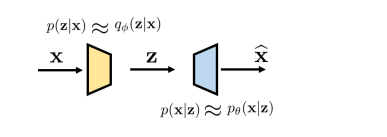
\includegraphics[width=1.25\linewidth]{sec/VAE_relation.png}
    \caption{In a variational autoencoder, the variables $\mathbf{x}$ and $z$ are connected by the conditional distributions $p(z|\mathbf{x})$ and $p(\mathbf{x}|z)$.}
\end{figure}
